\documentclass[12pt, authoryear]{elsarticle}
\makeatletter
\def\ps@pprintTitle{%
	\let\@oddhead\@empty
	\let\@evenhead\@empty
	\def\@oddfoot{}%
	\let\@evenfoot\@oddfoot}
\makeatother
%\usepackage{lmodern}
% My spacing
\usepackage{setspace}
\setstretch{1.5}
\usepackage{multirow}
%\DeclareMathSizes{12}{14}{10}{10}
\usepackage[margin=2.5cm]{geometry}    % How to set margins - optimized for 2.5cm

% See geometry.pdf to learn the layout options. There are lots.
\geometry{a4paper}                   			% ... or a4paper or a5paper or ...
\usepackage{enumitem}
\usepackage{mathtools}
%\geometry{landscape}                		% Activate for rotated page geometry
\usepackage[parfill]{parskip}    			% Activate to begin paragraphs with an empty line rather than an indent
\usepackage{graphicx}						% Use pdf, png, jpg, or eps§ with pdflatex; use eps in DVI mode
% TeX will automatically convert eps --> pdf in pdflatex
\usepackage{flafter}
\usepackage{setspace}
%\linespread{1.5}
\usepackage[font={}]{caption}
\usepackage[bottom]{footmisc}
\usepackage[capposition=top]{floatrow}   %figure notes
\usepackage{lscape}
%math packages
\usepackage{amssymb}
\usepackage{fancyhdr}
\usepackage{graphicx,epsf,subfigure}
\usepackage{pstricks,pst-node,psfrag}
\usepackage{amsthm,amssymb,amsmath}
\usepackage{amsmath,bm}

%mathnotes
\newcommand{\bbeta}{\mbox{\boldmath $\beta$}}
\newcommand{\beps}{\mbox{\boldmath $\epsilon$}}
\newcommand{\bX}{\mbox{\boldmath $X$}}
\newcommand{\bY}{\mbox{\boldmath $Y$}}
\newcommand{\bI}{\mbox{\boldmath $I$}}
\newcommand{\N}{\mathcal{N}}
\newcommand{\x}{\textsc{\textbf{x}}}
\newcommand{\xx}{\textsc{x}}

%add figure
\DeclareGraphicsRule{.tif}{png}{.png}{`convert #1 `dirname #1`/`basename #1 .tif`.png}
\usepackage{rotating}
\usepackage{pdflscape}
\usepackage{hyperref}
\usepackage[round]{natbib}
\usepackage{soul}
\graphicspath{ {../img/} }


\def\bibsection{\section{References}} %%% Make "References" appear before bibliography
\usepackage{longtable}
\usepackage{hyperref}
\usepackage{tablefootnote}
\usepackage{lscape}
\usepackage{animate}

\renewcommand{\contentsname}{Table of Contents} % change name from Contents to Table of Contents

\usepackage{titlesec}

\setcounter{secnumdepth}{4}

%_______________________________________________________________________________________________________%
%_______________________________________________________________________________________________________%
%\usepackage[table]{xcolor}% http://ctan.org/pkg/xcolor
%\usepackage{graphicx,multirow}
\usepackage{xcolor,colortbl}
\usepackage{xcolor}
%\usepackage{graphicx,multirow}
\usepackage[capposition=top]{floatrow}
\setcounter{secnumdepth}{4}
\usepackage{tikz}
\begin{document}

\begin{frontmatter}  %

\title{What are the Trolls up to?}


\author[Add1]{Felix Adam}
\ead{felix.adam@barcelonagse.eu}

\author[Add1]{Jordi Serra}
\ead{jordi.morera@barcelonagse.eu}

\author[Add1]{Sebastian Wolf}
\ead{sebastian.wolf@barcelonagse.eu}

\address[Add1]{Barcelona Graduate School of Economics, Barcelona, Spain}

\begin{abstract}
\small{
Abstract to be written here.
}
\end{abstract}

\vspace{1cm}

\begin{keyword}
\footnotesize{
Textmining \sep Russian Interference \sep Polarization  \\ \vspace{0.3cm}
%\textit{JEL classification} L250 \sep L100
}
\end{keyword}
\vspace{0.5cm}
\end{frontmatter}

\headsep 35pt % So that header does not go over title
\section{Introduction}\label{intro}

In this report we analyze efforts by the Russian Internet Research Agency (IRA) to polarize the American public on social media / twitter in the context of the 2016 presidential election. The 2016 election featured two candidates that bore starkly different promise for the Russian government. Whereas Hillary Clinton had already built her profile as a strong critic of Russian foreign policy during her tenure as Secretary of State, Donald Trump offered the opportunity for Russia to push American politics into a more favorable space for Russian interests. The topic has caused a lot of controversy in American politics over the last two years. Recently, the finally released, heavily redacted Mueller report has rekindled the debate, and provided evidence that Russia did indeed attempt to aid Trump's election, as had already been alleged by many political observers. Polarization likely played an important role in Russia's strategy to do so. Given Trump's more radical policy positions, a polarized society can be expected to play in his advantage, allowing him to increase his vote at the extremes of the political spectrum. Polarization might also have been a goal of the Russians in and of itself, by weakening American influence in world politics, and lowering faith in democratic vs autocratic political systems.

Any democratic government has a strong interest in counteracting such foreign interference in the national debate that can destabilise the democratic process. Therefore, there is strong policy justification for research into measures that help to identify polarization in twitter data. In this report, we attempt to do just that. We study a dataset of nearly 3 million tweets by user accounts linked to the IRA and use textmining techniques to uncover targeted efforts to polarize the national debate. To identify polarization, we propose to study the clusteredness of tweets. To do so, we project tweets onto a vector space created using the Word2Vec algorithm. We consider a corpus to contain polarizing tweets if the clusters that we find feature data points that have strong similarity within and low similarity across clusters. We measure this similarity using cosine distance of the word embedding vectors, and take high average pairwise distance between clusters and low average distance within clusters as a sign for polarization.

We acknowledge that clusters in our dataset cannot be expected to be perfectly separated, or bunched into a specific number of clusters. To build up credibility among the American public, IRA tweets needed to build a history of realistic tweets to increase followers and be taken seriously. We hence expect the dataset to feature a lot of noise, but still show larger across-cluster distance than the average Twitter corpus. In our empirical analysis, we study polarisation as evidenced by clusteredness both for the corpus as a whole and for individual topics as identified by hashtags. Our results show that XXXXXX

In the second section of this report, we clarify the likely political motivation of the Russian government to engage in a polarization strategy. The third section introduces our methodology. The fourth section describes the data and our pre-processing steps. The fifth section reports the results, and the sixth section discusses our conclusions.

\section{The Strategy behind Russian Social Media Efforts}\label{literature}

In order to identify efforts to polarize US politics through social media, we need to understand the strategies behind such efforts. In particular, it is crucial to know why Russia would use such strategies, and how they could potentially influence domestic and foreign politics in the US.

Unlike the predicted "End of History", (\cite{fukuyama1989end}) conflicts between liberal democracies in the west and Russia reemerged in the beginning of the 21st century. Following the fall of the Soviet Union, instead of integrating into the West, Russia tried to reestablish it's position as a superpower. Issues like the NATO integration of eastern European countries or the establishment of a missile defense shield in easter Europe lead to rising tensions and mistrust of Russian leaders towards the West (sources). These tensions became more pronounced in the beginning of the second decade of the 21st century, with hot conflicts in the middle East, most notably Syria, and the Maidan Revolution in Ukraine. At the heart of these conflicts were and still are diverging interests of the United States and Russia. Be it the integration of the Ukraine into the European Union (EU) and NATO or the Russian support for the Syrian leader Assad. These points of conflict can be seen as a motivator for the Russian interference in the 2016 US presidential elections.

In the aftermath of the 2016 elections, the US intelligence community published a number of assessments of the Russian strategy. Most notably, the Central Intelligence Agency (CIA), the Federal Bureau of Investigation (FBI) and the National Security Agency (NSA) published an assessment of Russian activities, stating that the goals of Russia were to weaken public faith in the US democratic process and denigrate presidential candidate Hillary Clinton (\cite{office2017assessing}). The idea behind these efforts was to undermine the US-led liberal democratic order, posing a threat to Putin's regime. In particular, Putin saw a potential presidency of Hillary Clinton as a threat to his ambitions in Ukraine and Syria, due to Clinton's foreign policy positions as Secretary of State. Trump on the other hand was seen more friendly towards Russia and thus favoured over Clinton. As part of these efforts, Russia used social media networks like Facebook and Twitter, to promote radical discontent with US politics, polarize the discussion and denigrate Hillary Clinton. The report further states, that the Russian strategy changed over time. In the beginning, the goal was to undermine public institutions. However, with Clinton leading over Trump, the Russian efforts shifted towards the defamation of Clinton, trying to harm her electability and potential presidency. Interestingly, the report states that after Trump had won, the efforts to undermine public institutions stopped. The three intelligence agencies pick out the so called Internet Research Agency (IRA), as one of the main sources of these social media accounts. The IRA is described as a private agency with ties to the Russian government, engaging in targeted social influence efforts.
The findings of the so-called Mueller investigation (\cite{mueller2019report}) support this assessment. According to the Mueller Report, the IRA carried out social media campaigns to amplify social discord in the US. In order to do so, Twitter accounts linked to the IRA tweeted on divisive US political and social issues, such as illegal immigration and racial injustice. According to \cite{mueller2019report}, the IRA used social media accounts in two manners. Some accounts were designed around fictitious US personas, posting original content on divisive topics, promoting radical ideas and denigrating or promoting political candidates. Other accounts weren't used for original content, but rather to promote and amplify the impact of the "original" content. Some of the  accounts posting such content had a large follower share, such as \@TEN\_GOP, an account pretending to be related to the Tennessee Republican Party. \@TEN\_GOP was clearly used to promote polarization by pushing extreme content and promoting Donald Trump. Some tweets included:

\begin{itemize}

\item "White girl burned alive by Black gang members  They should pay! Why media remains silent?"

\item "Wake up America before it's too late! Europe has already lost its chance!  \#BanIslam \#StopIslam \#filibuster"

\item "Donald Trump: "I will be the greatest jobs-producing president that God ever created"

\end{itemize}

The strategy clearly worked, since tweets of the IRA we're picked up by major news outlets in the US and thus shaped at least daily discussions (\cite{mueller2019report}). We can thus summarize the Russian strategy as follows: Polarize the political discussion in the US, undermine Clintons authority and electability and promote Trump.

Now the question remains how these strategies, if successful, would affect US foreign policy, in particular towards Russia. In the subsequent analysis, we'll focus on the idea of polarization. \cite{fiorina2008political} define polarization as the simultaneous presence of opposing or conflicting principles, tendencies or points of view. In a quantitative manner, polarization can be seen as an increase of variance of ideas and attitudes towards poltical questions. \cite{dimaggio1996have} argue, that this reduces the probability of group formation at the center of the political spectrum and increases the formation of groups with irreconcilable preferences. This can have peculiar effects on domestic and foreign policy. \cite{beinart2008politics} argues that polarization leads to a weakened international position of the US. First, international endeavours such as the promotion of trade agreements, UN resolutions or even military campaigns crucially depend on domestic support. Without domestic support, international allies of the US discount promises, while the US appears weak towards enemies \citep{beinart2008politics}. \cite{schultz2017perils} supports these findings. He argues that domestic political polarization leads to three issues. First, it is more difficult to get bipartisan support for risky undertakings. Second, it gets harder to agree on lessons from failures, complicating efforts to learn. And lastly, the risk of dramatic policy swings complicates the ability to make long term commitments. The overall effect of polarization can thus be summarised as follows: A polarized society is caught up with fighting against itself. It can't
reconcile large differences to find a common foreign policy strategy.

Consequently, Russia's global standing would greatly increase from a polarization of US politics. Actually, we can already see these effects in motion, especially in Syria. The US failed to gather international support for UN resolutions and seems to have no clear strategy, while Russia continues pushing its ally Assad \citep{bolan_2019}. Interestingly, the other strategies described by Martin and Shapiro, such as defamation and persuasion can also be seen as tools of polarization.

Having discussed the effects of polarization, we can now try to identify Russian polarization efforts through social media.

\section{Methodology}

Informally, polarization in society can be defined as a situation where we have high within-group similarity, and low across-group similarity. More formal measures have been proposed, for example by \cite{duclos2004polarization}, that relate specific characteristics of density distributions to polarization, and provide a more thorough treatment of the concept. But for our purposes the informal definition shall suffice. More importantly, we note the close relationship between polarization and clustering techniques in the field of unsupervised learning, or community detection in the field of network science. Clustering techniques in the field of unsupervised learning aim to detect data points that naturally belong together because they are close by some measure in some higher dimensional space, and that are far from other data points by that same measure. Similarly, in network science we try to detect communities of nodes that display high similarity in terms of their links. Nodes that form a community share many common friends, and they share very few common friends with nodes outside of their community. Essentially, polarization is the social science term to describe clustering of data points. This means that to detect polarization we can employ unsupervised learning methods to detect clusters, or network science tools to detect communities.

In this report we aim to make use of this insight by attempting to identify clusters in the body of tweets which could provide evidence of Russian efforts to polarize the American society ahead of the 2016 presidential election. A priori, the most natural clusters we would expect to emerge are two: one cluster pulling the debate towards the extreme left, and another cluster pulling the debate towards the extreme right. However, this would not be the only type of clustering that would yield evidence for polarization. Russian polarization efforts may also have been organized along topic lines, creating two or more clusters within a chosen set of topics. Further, any effort to polarize the debate would have to be hidden among a cloud of noise in order to conceal orchestrated nature of the effort, and to appear like a body of real tweets to the American twitter users. Therefore, we do not expect the clusters to yield perfect class separation, or yield very clear separation of opinions on topics. In support of our hypothesis we would expect that, compared to a non-orchestrated discussion on Twitter, the IRA tweet corpus shows more pronounced clustering. Similarly, the level of clustering should be comparable to what are known to be very polarized debates, for example the discussion among fans ahead of a football match of two rival teams.

Since tweets are completly unstructured text documents, clustering them as is will be impossible without any labels. We therefore make use of word embeddings, to represent each tweet in a continous vectorspace. In order to do so, we use the Word2Vec algorithm proposed by \cite{mikolov2013efficient}. The idea behind Word2Vec is to train a neural network on the corpus at hand, with the goal in mind of either predicting the sorrounding words of a given word (CBOW-architecture), or a word based on it's neighbors (skip-gram-architecture). In this setting we choose to train the network using the skip-gram architecture, hoping that we will capture the context in which a word is being used, allowing easier clustering. In the skip-gram set-up, the neural network has an input layer of one node which takes the current word as input. The goal is then to predict the $n$- neighboring words based on the input. Having trained the model, one can use the learned weights as a representation for each word. One can think of these word embeddings as describing a word by the company it keeps. Words that appear more often in the same context, will "point" towards a similar direction in the vector space. 

Having found word-vector, we can embedd the tweets by adding each word of a tweet and normalizing the resulting vector by it's norm. By doing so we hope to achieve two goals: First, tweets that are talking about similar topics, should be represented by a similar vector, thus enabling clustering. Second, we can find out how people talk about a given topic. For example, the words "good" and "bad" should be fairly dissimlar to each other, so tweets talking about "good" or "bad" politics should be differentiable inside said topic. 

To cluster the tweets we use the DBSCAN algorithm \cite{ester1996density}. Compared to partitioning based algorithms like k-means, DBSCAN aims to find clusters of high density. 
How DBScan Works: (JORDI TBD)
Minimum density level estimation, based on a threshold for the number of neighbors, $minPts$ within the radius $\epsilon$ with an arbitrary distance measure
Objects with more than $minPts$ neighbors within this radius are considered core points
The intuition behind DBSCAN is to find the areas which satisfy the minimum density and which are seperated by areas of lower density
All neighbors within the $\epsilon$ radius of a core point are considered to be part of the same cluster as the core point ("direct-density-reachable")
If any of these neighbors is again a core point, their neighborhoods are density reachable
Non-core points are called border points and all points within the same set are density connected
Points which are not density reachable from any core point are considered noise and do not belong to any cluster

<<<<<<< HEAD
To measure the level of clustering, we propose to use the average cosine distance between tweets. Other measures, such as the distance between the centroids, or the distance between certain quartiles, could also be considered, but we restrict ourselves to the average distance as this captures the across-group separation very well, giving the same weight to all tweets. Since our scope in this report is limited, we attempt to argue for polarization without comparing the average cosine distance we find in the IRA tweet corpus to other corpora, even though that would have been our preferred approach had we had more time. Instead, we check how close the average cosine distance is to the maximum theoretically possible distance (the cosine distance ranges from 1 to -1, with 0 being the largest distance).
=======
Compared to partitioning based algorithms like k-means, DBSCAN aims to find clusters of high density. The intuition behind DBSCAN is to find the areas which satisfy the minimum density and which are separated by areas of lower density. Objects in these sparse areas - that are required to separate clusters - are usually considered to be noise and border points. Formally, the algorithm is structured around core points. A point is considered core if there are more than $n_min$ neighbors at distance smaller than $\epsilon$. All neighbors that are at distance smaller than $\epsilon$ from a core point are considered to be part of the same cluster as the core point. Points that are not reached by any core point are considered to be border points and are not assigned to any cluster. $\epsilon$ and $n_min$ are tuning parameters of the algorithm.

The algorithm allows the use of multiple distance measures. In our case, for simplicity, we picked euclidean distance. We are aware that high dimensional spaces as ours can lead to "curse of dimensionality" problems and in future research we would consider other methods suited for high dimensional spaces.

Ideally, after finding the topics or clusters, we would like to find two separate groups within the cluster talking about the same topic but with completely different opinions. In other words, polarization. To measure the difference of opinions within topic/cluster, we propose to use the average cosine distance between tweets.
>>>>>>> fe917e4c3902c4c79acf7c71e2b8d6cb2f77e371

\section{Data}\label{data}
To identify efforts by Russia to polarize public opinion on social media ahead of the 2016 US presidential election, we make use of a dataset of nearly 3 million tweets by 3077 different English-language user accounts linked to the Internet Research Agency and made publicly available by Twitter covering several years leading up to and after the election period.

\subsection{Data preprocessing}

Preprocessing of the tweet corpus is of capital importance when using natural language processing techniques where different approaches in text cleaning/filtering can lead to starkly different results during model training. In this section we are going to describe and justify the steps we followed to clean our data.

\subsection{Filtering}

In the data set, we find tweets in different alphabets: latin, cyrillic and arabic. The first step we take is to remove all tweets that do not use the latin alphabet. We keep English tweets only. Besides not being able to extract any meaning from other alphabets without translation, having different languages/alphabets in the corpus can lead to wrong algorithm output and false vocabularies. Further, since the main target is to show the polarization caused by these tweets in the American society, we believe English is the most relevant language for this objective. We also drop users that don't have their user description or account language in English. Supposedly, having any of the features described above would look suspicious to the "true" American users who these accounts aimed to influence leading to counterproductive effects. After removing all these tweets from our data, we keep roughly 85\% of the original data set, which means 2.5 million tweets.

\subsection{Cleaning}

Tweets are usually data dirty: punctuation signs are used to structure the tweet, urls, retweets, hashtags and emojis are frequent. Cleaning of symbols that cannot be used to convey meaning in the embedding algorithm is key to obtain sensible results. We proceed by removing mentions, retweets, urls, breaklines and  blank spaces. A question that arises when analysing tweets is what to do with emojis. Generally speaking, emojis can be difficult to process but they carry important information about the tweet. In our case, after some preliminary results, we find that emojis don't help much on identifying polarization and, therefore, we removed them from our corpus.

Another important cleaning decision regards hashtags. Hashtags provide useful information for identifying the topic and a user's opinion about that topic. Since we want to identify polarized information, we believe that these hashtags yield important information in identifying polarization, so we keep them as hashtags in the corpus.

\subsection{Further preprocessing}

A classical approach for data cleaning in text-mining is to follow the Stop Words - Stem - Lemmatize - Tokenize pipeline. However, in the case of short texts such as tweets, some recent contributions \cite{preprocessing} have argued that lemmatization and stemming lead to worse performance in terms of sentiment analysis, while feature reservation, negation transformation and repeated letters normalization improves it. Other references such as \cite{Hollink2004} support the view that lemmatizing and stemming does not improve performance of the algorithms significantly. One has to keep in mind that any morphological pre-processing of the training data reduces the amount of information that model can obtain from the corpus, which can create unnecessary noise making some sentences ambiguous. Therefore, since there is no clear evidence that we can improve performance using lemmatization and stemming, we prefer not to add this layer of complexity to the problem and stick to the cleaned tokenized raw data.

\subsection{Data exploration}

According to \cite{mueller2019report} Russia deployed a complex strategy to influence American elections through an army of troll tweeter accounts. Our hypothesis is that this was done via three main channels: politically active users, fake news accounts and bot accounts. We will call the first two channels the content providers and the third channel the content amplifier. The politically active accounts are well identified in the reports by the American intelligence agencies and also by their user descriptions. The news providers consist in a few number of users that attempted to impersonate local news agencies and spread both true and fake news. The idea behind is that, in order to get a loyal audience, they had to build up credibility providing real news for a wide range of topics. However, among these "innocent" news they also published tweets with highly polarizing socio-political content. These content provision interventions appear to then have been complemented using bot twitter users to amplify the content from content providers via retweets.

\subsection{Content creators vs content amplifiers}

In order to verify the underlying phenomena introduced previously we plotted the percentage of retweets per user in figure \ref{retweets:1}. We find that there is a clear separation of roles: the amplifier is a user with a high percentage of retweets who only retweets information from other users. The content creator is a user with low percentage retweet percentage, only creating content.

\begin{figure}[t]
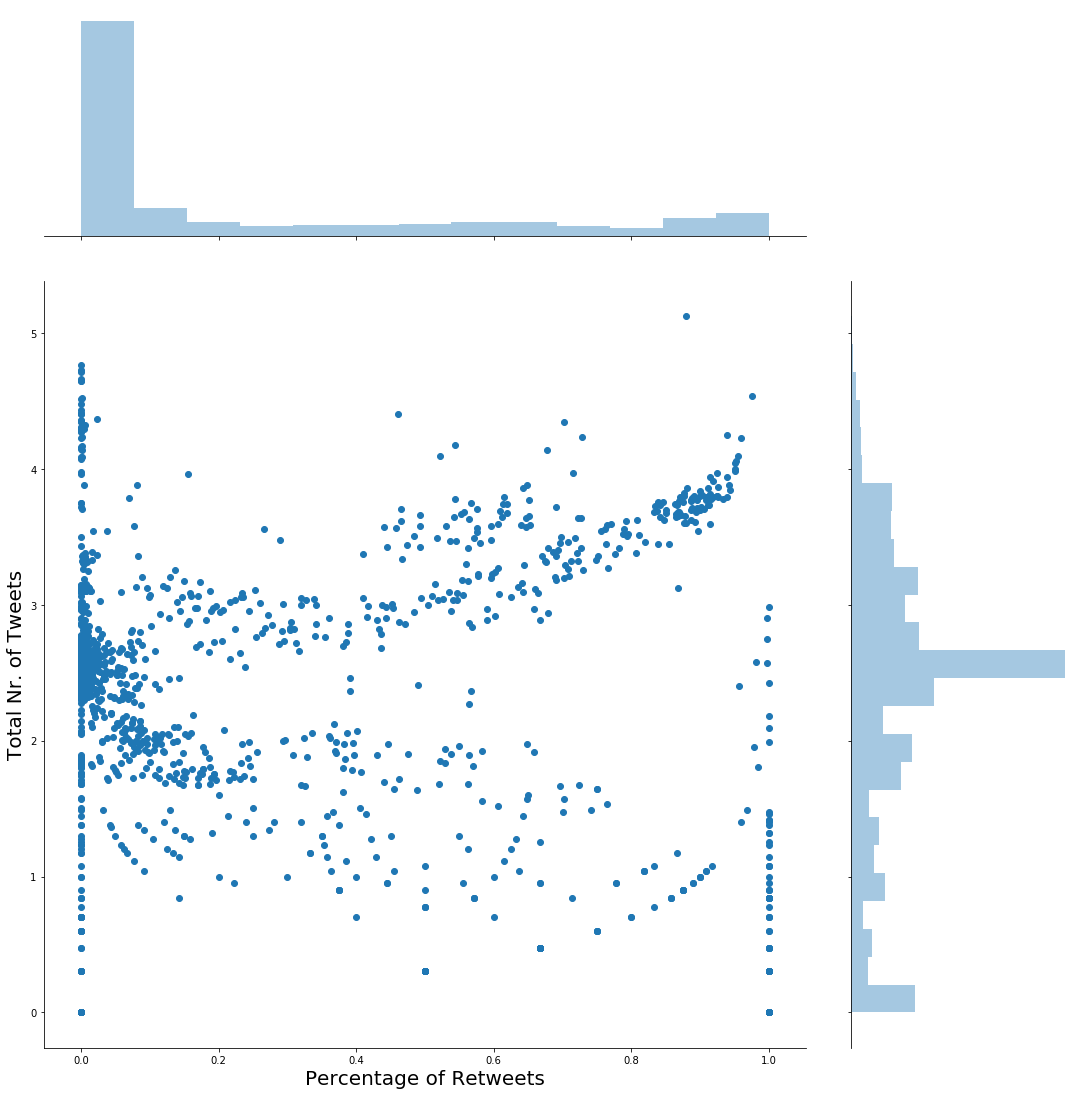
\includegraphics[width=\textwidth]{retweets}
\centering
\caption{Retweet ratios}
\label{retweets:1}
\end{figure}

In the upper right corner of figure \ref{retweets:1}, we see a high concentration of users that, despite having a large total number of tweets, hardly ever produce any content. On the other extreme we have users that produce a reasonable amount of original content tweets but hardly ever retweet. We identify an outlier that has more than 150.000 tweets, which means that over 5 years of data, this user was retweeting an average of 80 tweets per day! The plot also features some interesting 'curves' that make up perfect lines. This appears like clear evidence for bots created 'at scale' with varying retweet percentages programmed using a specified retweet/total tweet function.

We identified the most politically active accounts and it seems that, as expected, all of them fit in the content provider category. Find the retweet ratio of these users in table \ref{table:1} and \ref{table:2} in the Annex, already classified by left-wing/right-wing partisans. Also, as we can see in table \ref{table:3} and \ref{table:4} in the Annex, that their user description already gives a clear idea of their political beliefs. Regarding news providers, having an average of retweet ratio of 0.01 we can also confirm that they fit in the content provider category.

As an exploratory step, we have checked the content providers' most frequent used words and produced wordclouds for them (see Annex). In figure \ref{wordcloud:1} we clearly see the preferences of right-wing partisans, mainly talking about Obama and religion related topics. In figure \ref{wordcloud:2} we can clearly see the topics left-wing partisans talk about.  Note, for example, a considerable amount of anti-racism vocabulary. Finally, for news providers in figure \ref{wordcloud:3}, we cannot identify any more a political preference nor extreme vocabulary but just a normal vocabulary a news provider would use.

\begin{figure}[t]
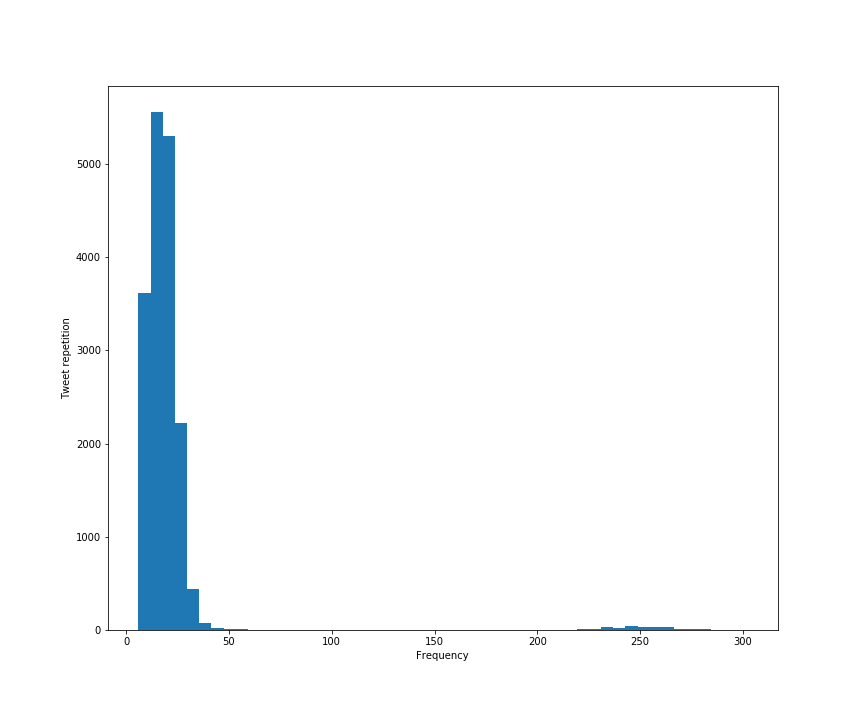
\includegraphics[width=\textwidth]{tweet_rep}
\centering
\caption{Repeated tweets}
\label{retweets:2}
\end{figure}

\subsection{Repeated tweets}
Deepening into tweet text exploration we perceived identical tweets from different users that have not been retweeted. In other words, different users posted the exact same text several times. In figure \ref{retweets:2} we plotted the distribution of how many repetitions we have from a tweet excluding retweets. We see a high concentration of repeated tweets below 50 repetitions and then a small concentration again around 250 repetitions.A first look at the tweet text suggests that more frequent tweets seem to be talking about self-aid and motivation sentences whereas the less frequent tweets seem to be news repeated by the news providers.

A possible explanation for this scenario is that content amplifiers or bots don't have a retweet ratio of exactly 0. Which means that, at some point, this bots have "created" some content. Therefore, they make use of a pool of motivation sentences to "create" tweets so they don't arouse suspicion.
This is a particularly notable results since the repeated tweets are almost 30\% of the "original" created content.

\subsection{Hashtags}
As explained previously, hashtags are relevant when analysing tweeter data since they perform as a good proxy for the topic of tweet. In figure \ref{wordcloud:4} and \ref{wordcloud:5} we plot most repeated hashtags among all the available data for left and right partisans. In general, users with different political convictions don't share hashtags. This is because, usually, a hashtag has inherently a political belief behind and using it presuppose that the user is in favor of that belief. There is one particular exception with the hashtag "BlackLivesMatter" which is relevant in both groups. Apart from that, we do no see any other important information for our study.

\section{Results}

Having cleaned the data of non-english tweets and users, we trained the Word2Vec algorithm using Pythons Gensim library \cite{rehurek_lrec}. We trained the algorithm on the full corpus, using a skip-gram archtiecture with a window size of 4, embedding the tweets into a 100 dimensional subspace.

Our results on individual words show promosing results towards the polarizing nature of some of these tweets. Tables \ref{table:1} and \ref{retweets:2} show the most similar words to Trump and Clinton

In Figures \ref{embedding:1}, \ref{embedding:2}, \ref{embedding:3} and \ref{embedding:4} we see a lower-dimensional visualization of some word vectors, created using the t-SNE algorithm \cite{pmaaten2008visualizing}. Each plot shows the comparison of two words in orange and light-blue and their 10 most similar words as measured by the cosine similarity of the vectors. In Figure \ref{embedding:1} we can already make out some strinking differences between the similar vectors for Liberals and Conservatives. In a normal context, one would expect the word "Liberals" to be close "Conservatives" or other words describing the political spectrum. Here however we see, that the most similar words to liberal all seem to have a negative meaning, such as "Libtard", "Intolerant" and "Dishonest" or are connected to derogatory hashtags, like "Liberallogic". On the other hand, the similar words for Conservatives are much less extreme, highlighting the Russian bias towards Trump as a conservative candidate. We see similar results in Figure \ref{embedding:2}, where Clinton is connected to words relating scandals like the e-mail scandal. Another clear indicator of the polarization efforts can be seen in figure \ref{embedding:3}, highlighting the Russian efforts to polarize the society alongside racial injustice topics. In a normal corpus, we would expect "Black" and "White" to be similar to other colors. Here we see that they are mostly social justice based, with "Black" being similar to black rights and "White" being close to notions of privilige and racism.
As we can see in Figure \ref{embedding:1}

\begin{center}
\begin{table}[H]
\begin{tabular}{ c c }
Skip Gram - Word   &  Similarity \\
 \hline
donald   &  0.896358\\
trumps   &  0.791140\\
pres   &  0.770282\\
feedly   &  0.762091\\
illegitimate  &   0.755011\\
president   &  0.742422\\
trum   &  0.736769\\
administration  &   0.728688\\
donaldtrump   &  0.728006\\
rnc   &  0.725931\\
 \hline
\end{tabular}
\caption{Most similar words to Trump}
\label{table:5}
\end{table}
\end{center}

\begin{center}
\begin{table}[H]
\begin{tabular}{ c c }
Skip Gram - Word   &  Similarity \\
 \hline
hillary   &  0.935136\\
hillaryclinton   &  0.783674\\
clintons &    0.781306\\
hrc   &  0.765259\\
campaign  &   0.741458\\
sanders  &  0.738335\\
emails   &  0.724602\\
crookedhillary    & 0.723004\\
hillarys   &  0.721376\\
billclinton  &   0.717722\\
 \hline
\end{tabular}
\caption{Most similar words to Clinton}
\label{table:6}
\end{table}
\end{center}


<<<<<<< HEAD
Having seen how the polarization efforts materialize in word similarities, we tried to cluster the tweets, tryingg to find similar structures. Our first effort at finding two distinct "polarization" clusters using k-means with 2 clusters failed. Without removing the news accounts and retweeters, the clustering algorithm picked up these as distinct clusters, showing their overall importance for the Russian efforts. Being interested in the "content-creators" described in section \ref{data}, we removed retweets and re-appearing tweets, possibly arising from a pool of tweets used by bots to appear human. Removing these users reduced the size of our dataset substantially, leaving roughly 400.000 tweets. For efficiency reasons, we clustered a random subsample of 100.000 tweets, using DBSCAN with an $\epsilon$-parameter of 0.6 and a minimum neighbor count of 15, forcing many tweets into the "noise"-cluster. 
=======
Having seen how the polarization efforts materialize in word similarities, we tried to cluster the tweets, trying to find similar structures. Our first effort at finding two distinct "polarization" clusters using k-means with 2 clusters failed. Without removing the news accounts and retweeters, the clustering algorithm picked up these as distinct clusters, showing their overall importance for the Russian efforts. Being interested in the "content-creators" described in section \ref{data}, we removed retweets and re-appearing tweets, possibly arising from a pool of tweets used by bots to appear human. Removing these users reduced the size of our dataset substantially, leaving roughly 400.000 tweets. For efficiency reasons, we clustered a random subsample of 100.000 tweets, using DBSCAN with an $\epsilon$-parameter of 0.6 and a minimum neighbor count of 15, forcing many tweets into the "noise"-cluster.
>>>>>>> fe917e4c3902c4c79acf7c71e2b8d6cb2f77e371


We then used DBSCAN to discover

- we used the Word2Vec algorithm with skip-gram

As described previously,



\begin{figure}[t]
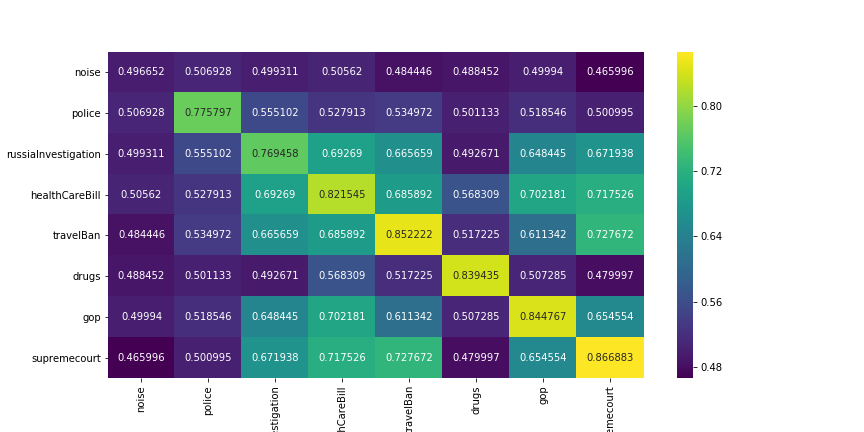
\includegraphics[width=7in]{heatmap_cluster_similarity}
\centering
\caption{Between-cluster distances}
\label{distance:1}
\end{figure}

\section{Discussion}

%_______________________________________________________________________________________________________%
%BIBLIOGRAPHY
%_______________________________________________________________________________________________________%
\pagebreak
\bibliographystyle{agsm}
\setcitestyle{authoryear}
\bibliography{textmining}

\clearpage

\section{Annex}

\begin{center}
\begin{table}[H]
\begin{tabular}{ c c } 
Twitter user name & Retweet ratio \\
 \hline
Jenn\_Abrams	&	0.0231\\
SouthLoneStar	&	0.0375\\
USA\_Gunslinger&	0.0770\\
patriototus		&	0.0033\\
redlanews		&	0.0038\\
 \hline
\end{tabular}
\caption{'Right' cluster retweet ratios among content providers}
\label{table:1}
\end{table}
\end{center}

\begin{center}
\begin{table}[H]
\begin{tabular}{ c c } 
Twitter user name & Retweet ratio \\
 \hline
BleepThePolice &   0.6768 \\
Blk\_Voice       &  0.0163 \\
KaniJJackson   &   0.2655 \\
LaChristie  &      0.0986 \\
gloed\_up       &   0.4606 \\
wokeluisa     &    0.0822 \\
 \hline
\end{tabular}
\caption{'Left' cluster retweet ratios among content providers}
\label{table:2}
\end{table}
\end{center}


\begin{center}
\begin{table}[H]
\begin{tabular}{ l l }
Twitter user name & User description \\
 \hline
USA\_Gunslinger &	Truth is strong, and sometime or other will prevail! \\
SouthLoneStar	& Proud TEXAN and AMERICAN patriot \#2a \#prolife \\
& \#Trump2016 \#TrumpPence16 Fuck Islam and PC. \\
& Don't mess with Texas! \\
patriototus	Being & patriotic means love or devotion to your homeland \\
& and readiness to defend it from any harm. United we stand, \\
& divided we fall. Conservative politics. \#PJNet \\
redlanews	& Conservative; Right and proud; Christian. Love my \\
& country and will stand against liberals and socialists. \\
Jenn\_Abrams &	Calm down, I'm not pro-Trump. I am pro-common sense. \\
& Any offers/ideas/questions? DM or email me \\
& jennnabrams\@gmail.com (Yes, there are 3 Ns) \\
 \hline
\end{tabular}
\caption{'Right' cluster profile descriptions}
\label{table:3}
\end{table}
\end{center}

\begin{center}
\begin{table}[H]
\begin{tabular}{ l l }
Twitter user name & User description \\
 \hline
Blk\_Voice & 	Activist. Feminist. Celebrating and highlighting Black excellence. \\
KaniJJackson &	Follow the example set by Mrs Obama; peace, love, acceptance \\
&  \& vigilance \#Impeach45 \#Resist \#GunReformNow \\
LaChristie	& Progressive. Activist. Warrior. Inspiration. \#Resistance \\
gloed\_up &	No black person is ugly \#BRONZE \#BlackLivesMatter \\
&  \#BlackToLive \\
BleepThePolice	 & For a second at least, I'm resurrecting the peace \#Blacktivist \\
& \#BlackLivesMatter \\
wokeluisa	& APSA. \#Blackexcellence. Political science major \\
 \hline
\end{tabular}
\caption{'Left' cluster profile descriptions}
\label{table:4}
\end{table}
\end{center}

\begin{figure}[H]
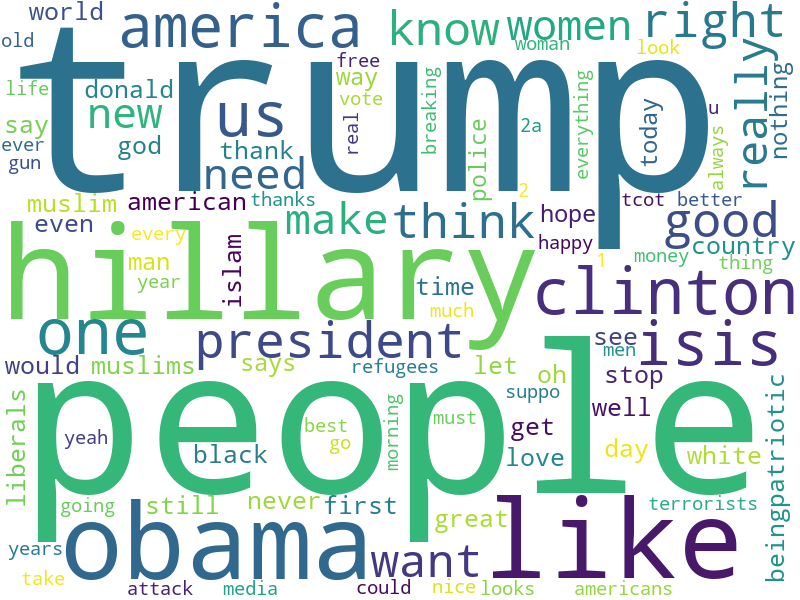
\includegraphics[width=5in]{wordcloud2}
\centering
\caption{Wordcloud for 'right' cluster}
\label{wordcloud:1}
\end{figure}

\begin{figure}[H]
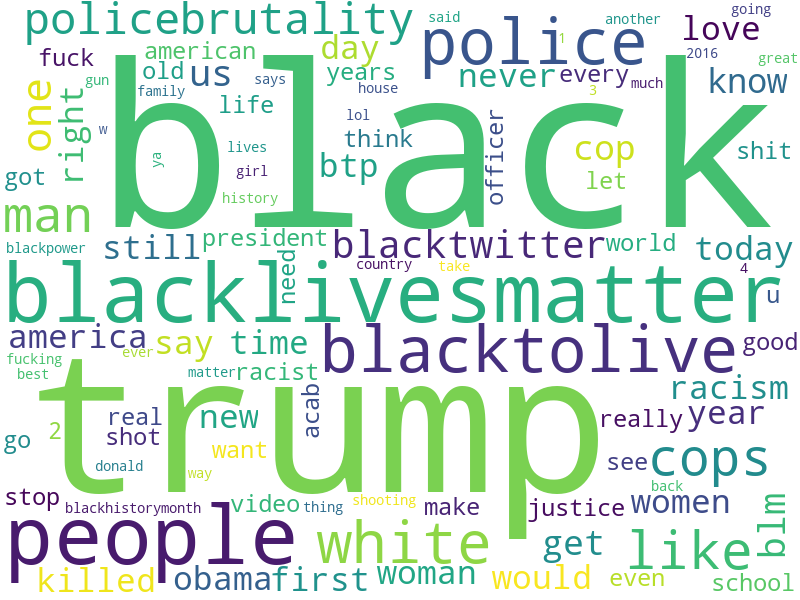
\includegraphics[width=5in]{wordcloud1}
\centering
\caption{Wordcloud for 'left' cluster}
\label{wordcloud:2}
\end{figure}

\begin{figure}[H]
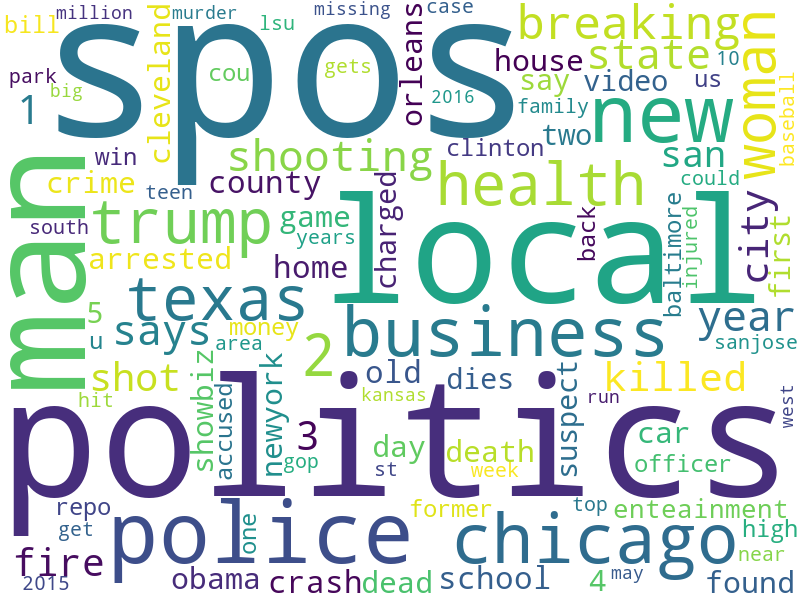
\includegraphics[width=5in]{wordcloud3}
\centering
\caption{Wordcloud for news providers}
\label{wordcloud:3}
\end{figure}


\begin{figure}[H]
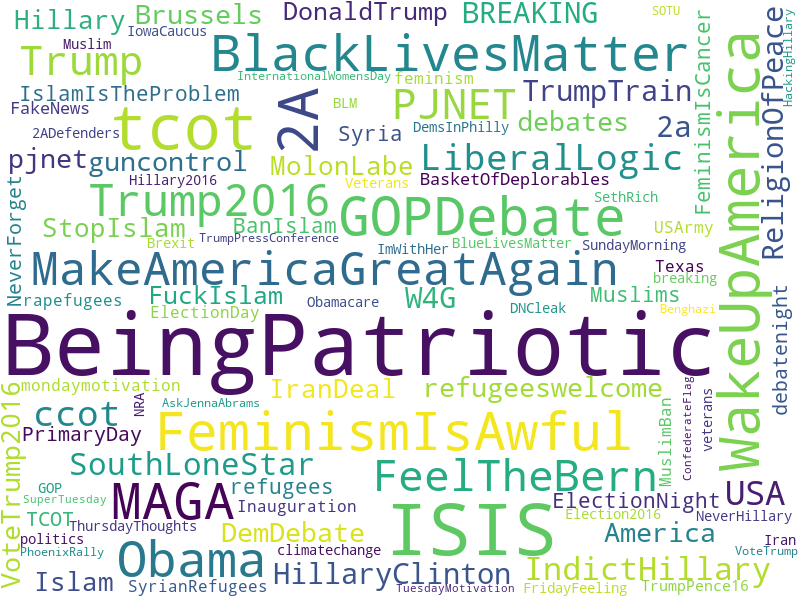
\includegraphics[width=5in]{wordcloud4}
\centering
\caption{Wordcloud 4}
\label{wordcloud:4}
\end{figure}

\begin{figure}[H]
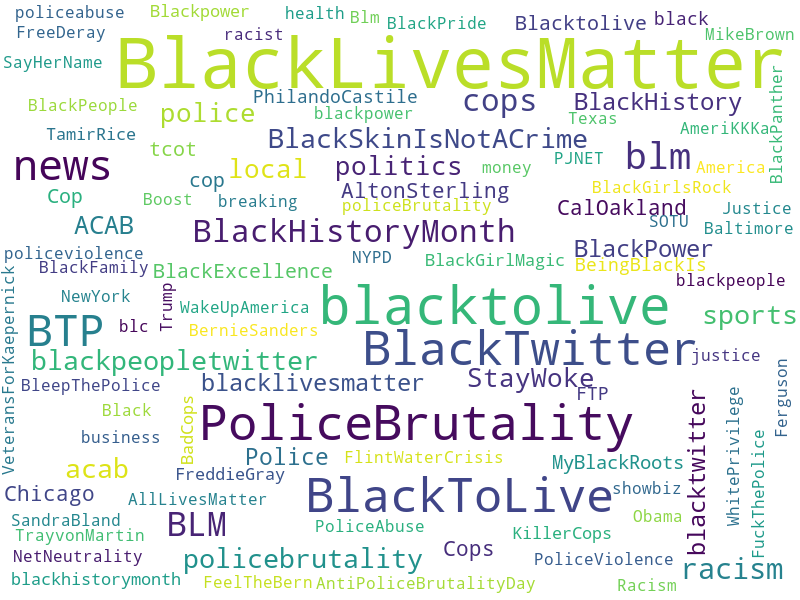
\includegraphics[width=5in]{wordcloud5}
\centering
\caption{Wordcloud 5}
\label{wordcloud:5}
\end{figure}

\begin{figure}[H]
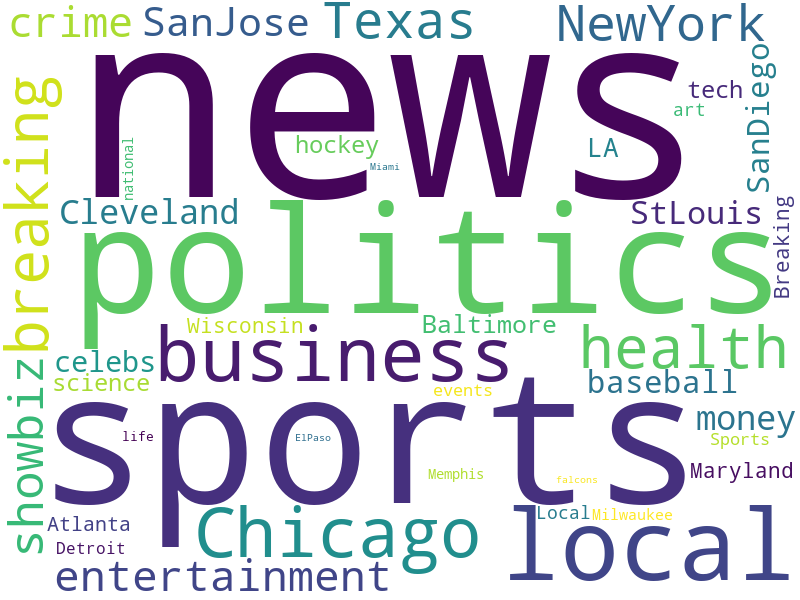
\includegraphics[width=5in]{wordcloud6}
\centering
\caption{Wordcloud 6}
\label{wordcloud:6}
\end{figure}

\begin{figure}[H]
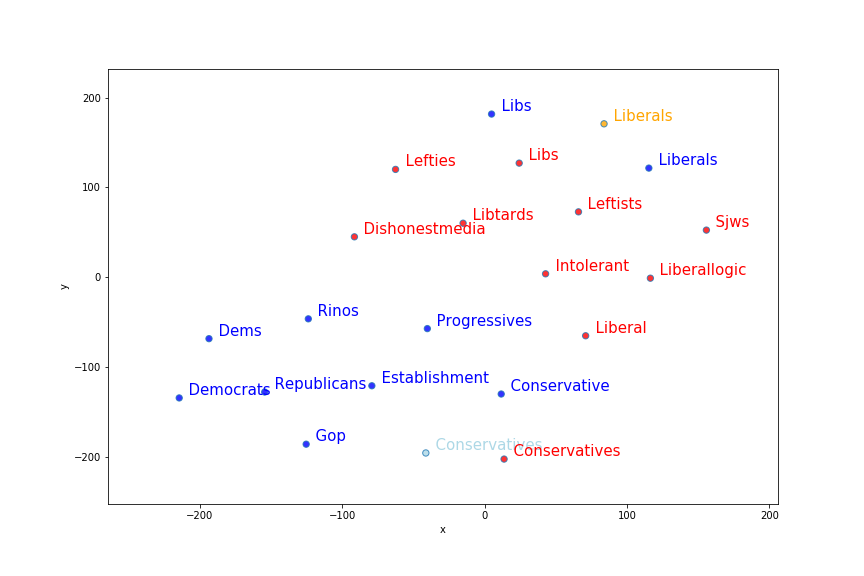
\includegraphics[width=6in]{embedding_liberals_conservatives}
\centering
\caption{Similarity of embedding: Liberals and Conservatives}
\label{embedding:1}
\end{figure}

\begin{figure}[H]
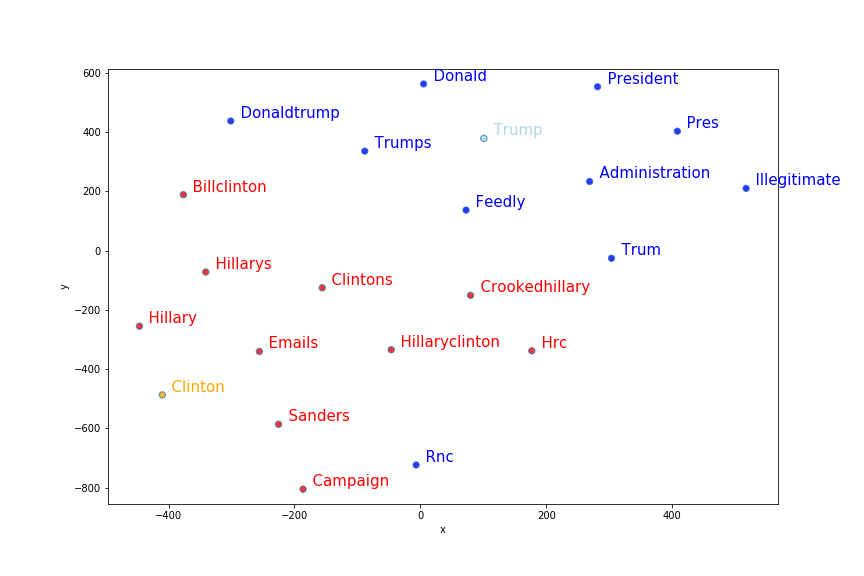
\includegraphics[width=6in]{embedding_clinton_trump}
\centering
\caption{Similarity of embedding: Clinton and Trump}
\label{embedding:2}
\end{figure}

\begin{figure}[H]
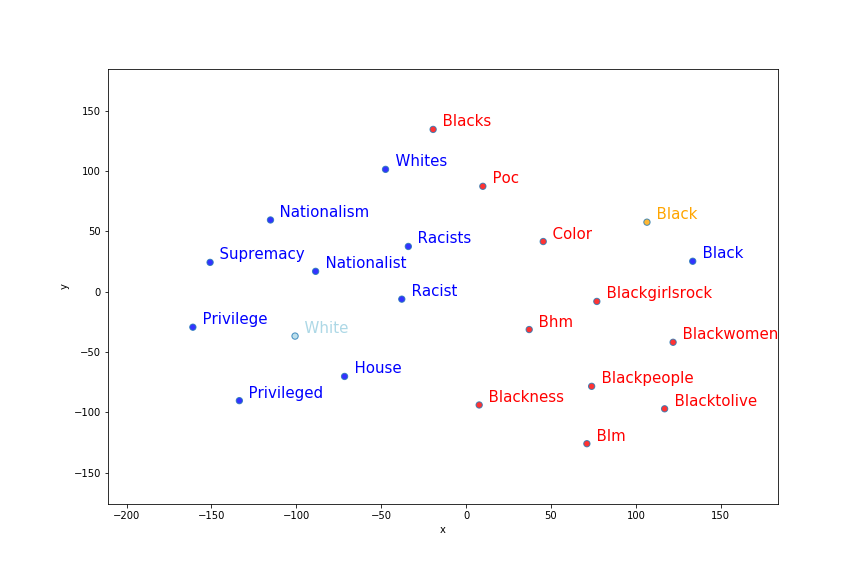
\includegraphics[width=6in]{embedding_black_white}
\centering
\caption{Similarity of embedding: Black and White}
\label{embedding:3}
\end{figure}

\begin{figure}[H]
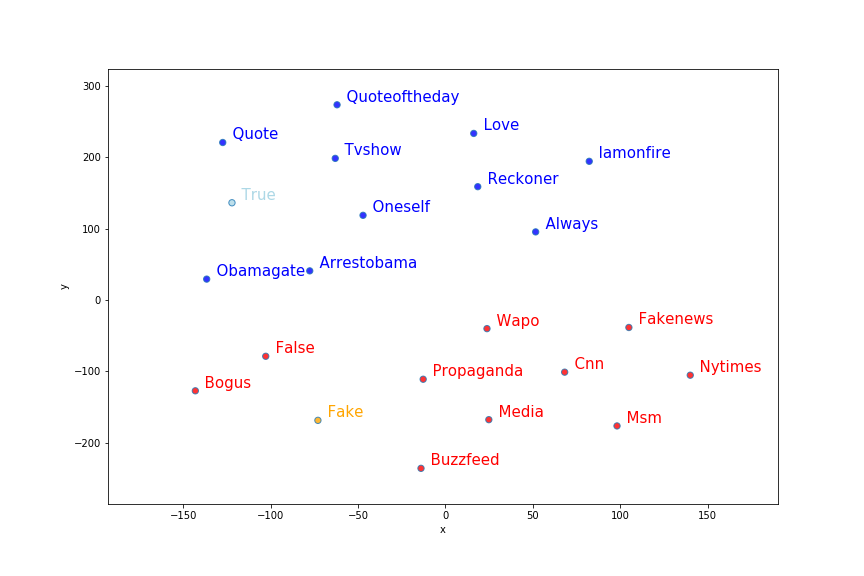
\includegraphics[width=6in]{embedding_fake_true}
\centering
\caption{Similarity of embedding: Fake and True}
\label{embedding:4}
\end{figure}

\begin{center}
\begin{table}[H]
\begin{tabular}{ c c }
Skip Gram - Word   &  Similarity \\
 \hline
liberallogic   &  0.760208 \\
nutshell   &  0.755933 \\
liberals   &  0.723288\\
msm   &  0.703458\\
hypocrisy  &   0.688949\\
communist  &   0.687983\\
leftists  &   0.671862\\
suppoers    & 0.671141\\
libs   &  0.670767\\
gopdebatesc   &  0.668273\\
 \hline
\end{tabular}
\caption{Most similar words to Liberal}
\label{table:7}
\end{table}
\end{center}

\begin{center}
\begin{table}[H]
\begin{tabular}{ c c }
Skip Gram - Word   &  Similarity \\
 \hline
republican    & 0.736253 \\
conservatives    & 0.693829\\
scprimary &    0.680811\\
 gop   &  0.673089\\
oppose   &  0.669254\\
cruz  &   0.656088\\
democratic  &   0.655370\\
democrats   &  0.654107\\
 convention  &   0.653456\\
endorses  &   0.648152\\
 \hline
\end{tabular}
\caption{Most similar words to Conservative}
\label{table:8}
\end{table}
\end{center}


\end{document}
